\documentclass{article}
\usepackage[margin=1.3in]{geometry}
\usepackage{lipsum}
\usepackage{multirow}
\usepackage{graphicx}
\usepackage{subfig}
\usepackage{float}

\title{Water Service platform for underserviced communities}
\author{Chang Liu, Sneha Das}

\begin{document}
\maketitle

\section{Introduction}
We developed an android application to address the ’crowd-
sourcing’ of the inspection and detection of water service malfunctions, in under-
resourced communities. The application has options for civilians, who wish to
report malfunctions and leakages, and plumbers to register with the KWSTF,
to provide timely services to repairs, based on standard remuneration. Thus,
this application is conceptualized to function as a mediator between the public,
who thrive to maintain the water services for the community, and the plumbers
available in the region. Not only does this accelerate the provision of services
for maintaining water infrastructure when resources are constrained, but it could also
helps in providing jobs and visibility to the plumbing community.

The application provides the users with two options: 1. to report leakages in the city 2. to provide plumber services. As a user reporting a leak, the app does not necessarily require the user to login or sign-up. However, a registered plumber with the KWSTF is required to have a profile which is made possible by signing-up and login-in to use the app, because based on the work history and feedback received by a plumber, their profile 
is updated, which adds a level of credibility of the plumber. The application begins with the home-page, mainly
comprising of two buttons, for {\it reporting} and {\it registering}. Also, if the user already has an account, they have 
an option to {\it login}. If the user wishes to report a leak, they choose {\it report}, which re-directs
them to the report form. This form requests all the details required to look for a plumber with potential 
to fix the malfunction. The user has options to {\it send report} or to {\it cancel} the action. If the user chooses {\it cancel}, they are taken to the home screen. On pressing
{\it send report}, a pop-up is presented to the user with confirmation that the report was sent. The user 
can dismiss the pop-up by pressing {\it OK} on the pop-up, following which the screen with details of the expected arrival time of the plumber is displayed to the user. This view is designed to contain a counter, which is indicative of the plumber's arrival. In the completely functional app, the counter should be initiated and controlled by backend-coding and search and find action by the KWSTF to locate a plumber. When a plumber is found, the corresponding details are also displayed on this screen. Finally, when the plumber
has fixed the issue, this information is updated to the user under {\it My report}. At any time after submitting the report, the user can access the status of the complain under {\it My report}. Also, in all the screens, a navigation screen is provided for users to go to the {\it Home}, {\it Setting}.

To register as a plumber, the user chooses {\it register} on the home screen, following which they are redirected to the registration form. this form seeks the basic details to evaluate the suitability of the plumber and the resource they can be. After submitting, the user is notified of the time the process could take and the contact details to get back to KWSTF. During the evaluation process, the plumber can stay updated
about the application status by visiting {\it My profile}. The possible outcomes of the registration request 
are {\it Pending}, {\it Approved}, {\it Rejected}. If the registration is approved, then the details provided by the user is saved as the user profile, work history. etc. The back-end procedure for registration should 
include a rigorous vetting process and security-check among other evaluation criterion. 



\section{Background}
In the design of the User-Interface, we have explored the following guidelines:
\begin{enumerate}
\item{\bf Four Principles of Good Design (Shneiderman 1998)}
\begin{itemize}
\item State and the action alternatives should be visible
\item Should be a good conceptual model with a consistent system image
\item Interface should include good mappings that reveal the relationships between stages
\item User should receive continuous feedback
\end{itemize}

\item{\bf Nielsen’s Ten Heuristic Rules (1993)}
\begin{itemize}
\item Simple and natural dialog
\item Speak the user’s language
\item Minimize user’s memory load
\item Consistency
\item Feedback
\item Clearly marked exits
\item Shortcuts
\item Good error messages
\item Prevent errors
\item Help and documentation
\end{itemize}
\item{\bf Jakob Nielsen’s Ten Usability Heuristics}
\begin{itemize}
  \item Visibility of system status (Feedback)
  \item Match between system and the real world (METAPHOR)
  \item User control and freedom (NAVIGATION)
  \item Consistency and standards (CONSISTENCY)
  \item Error prevention (PREVENTION)
  \item Recognition rather than recall (MEMORY)
  \item Flexibility and efficiency of use (EFFICIENCY)
  \item Aesthetic and minimalist design (DESIGN)
  \item Help users recognize, diagnose, and recover from errors (RECOVERY)
  \item Help and documentation (Help)
\end{itemize}
\item{\bf Shneiderman’s Eight Golden Rules}
\begin{itemize}
\item Strive for consistency
\item Enable frequent users to use shortcuts
\item Offer informative feedback
\item Design dialog to yield closure
\item Offer simple error handling
\item Permit easy reversal of actions
\item Support internal locus of control
\item Reduce short-term memory load
\end{itemize}
\item{\bf Smith \& Mosier: Data Display}
\begin{itemize}
\item 2.0/1Necessary Data Displayed
\item 2.0/2 Only Necessary Data Displayed
\item 2.0/3 Data Displayed in Usable Form
\item 2.0/4 Data Display Consistent with User Conventions2.0/6 Consistent Display Format
\item 2.0/8 User Control of Data Display
\item 2.0/12 Familiar Wording
\item 2.0/15 Consistent Grammatical Structure
\end{itemize}
\end{enumerate}

\section{Methodology}
The tools we are using includes design tools and software engineering tools.
For the design tools, we used paper and hand drawing to draw the framework of the initial pages, and then we organize
the initial pages together to a flow diagram, with a clear indication of how the pages are interacting with each other.
For the engineering tools, we used Android Studio to put the design we made into an android project. We used xml
language to define the layout of the page and then we used java language to create the function behind the layout.

\subsection{Guideline 01}
Four Principles of Good Design (Shneiderman 1998):\\
2. Should be a good conceptual model with a consistent system image.\\


\begin{center}
  \begin{tabular}{ |c|p{8cm}|  }
  \hline
  \multicolumn{2}{|c|}{\bf Implementation} \\
  \hline
  {\bf Content Items} & {\bf Style} \\
  \hline
  Page Title & 20sp, dark blue color \#4FC3F7, bold \\
  \hline
  Page content subtitle & 12sp, blue color, \#4FC3F7 \\
  \hline
  Page content plain text & 12sp, black color \#000000 \\
    \hline
  Buttons    & \parbox[t]{7cm}{background: blue color, \#81D4FA\\ text: 12sp, white color \#FFFFFF} \\
    \hline
  Text Links & 12sp, blue color, \#4FC3F7 \\
    \hline
  Input Text Box & background: light blue color, \#E1F5FE   \\
    \hline
  Dropdown list & background: light blue color, \#E1F5FE \\
    \hline
  Radio Buttons & 12sp, black color \#000000 \\
    \hline
  Contact card & background: light blue color, \#E1F5FE\\
  \hline
  \end{tabular}
\end{center}


\begin{figure}[H]
  \centering

\subfloat[label 1]{{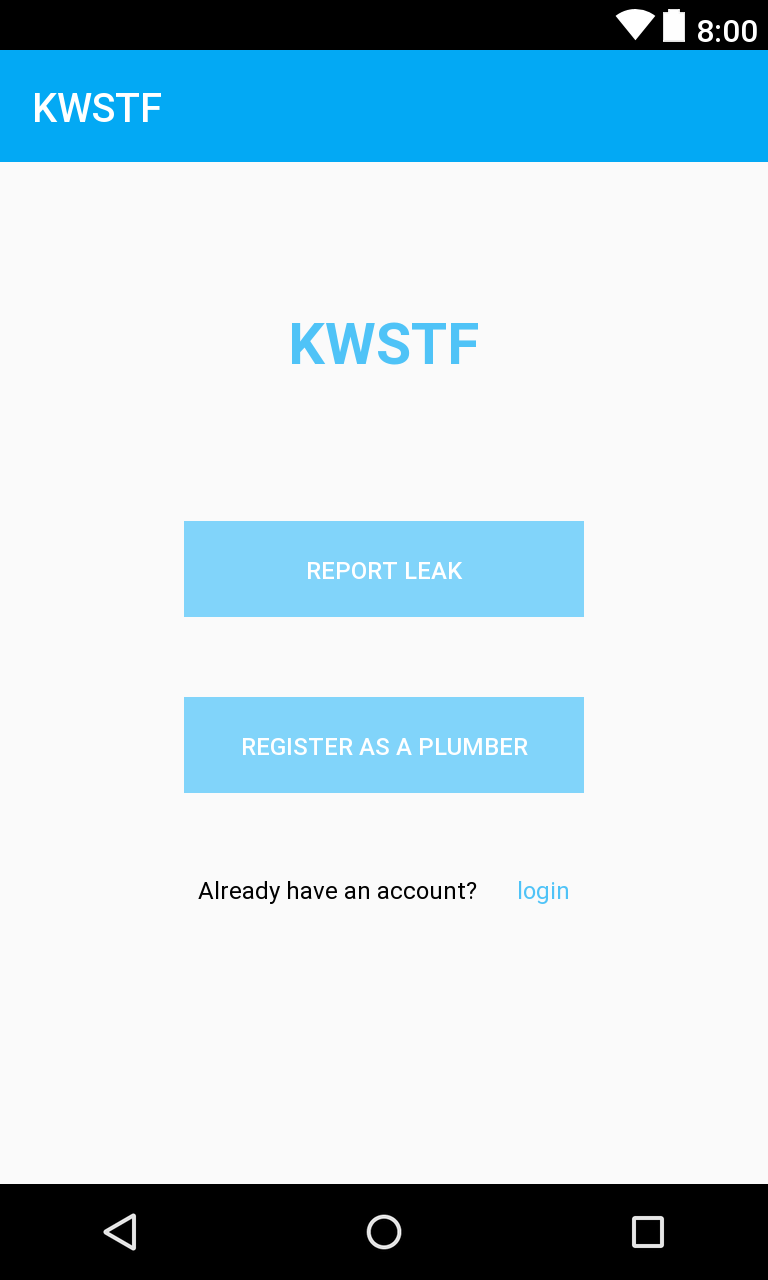
\includegraphics[width=4cm]{files/report_leak/home.png} }}%
\qquad
    \subfloat[label 2]{{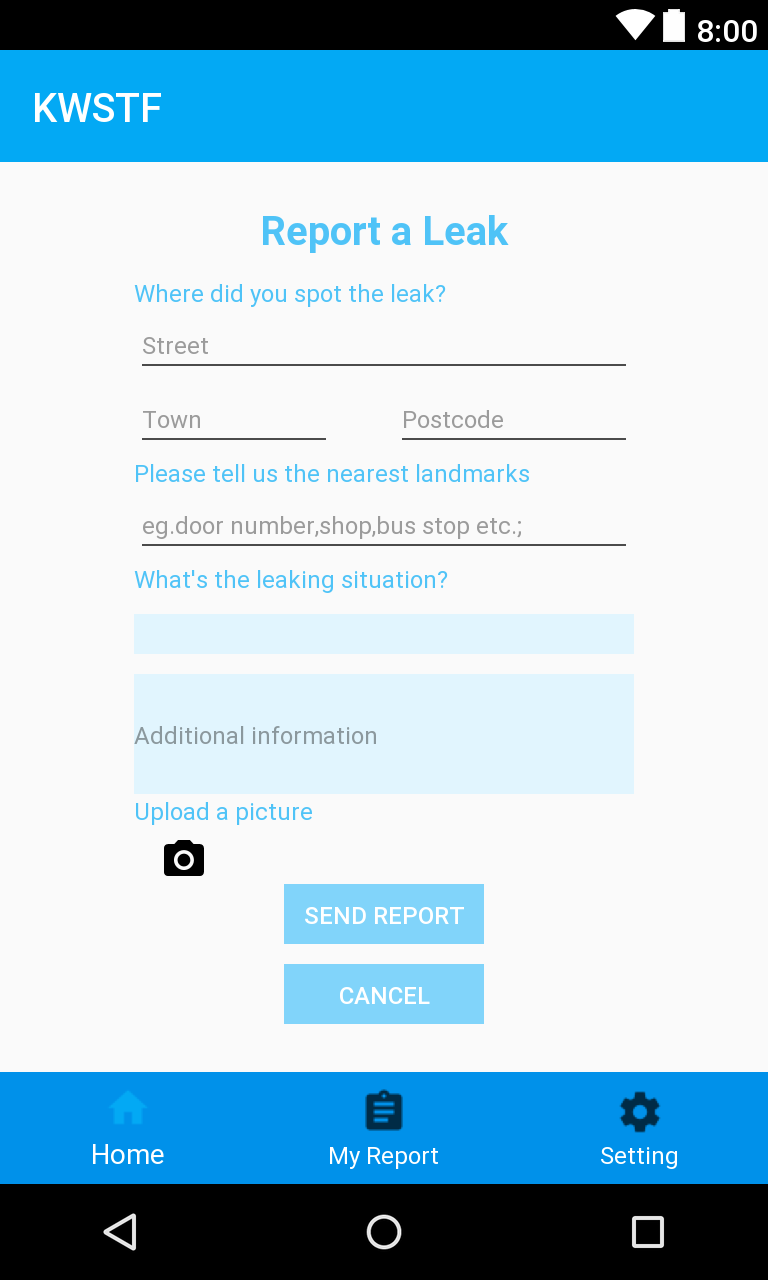
\includegraphics[width=4cm]{files/report_leak/a1.png} }}%
    \qquad
    \subfloat[label 3]{{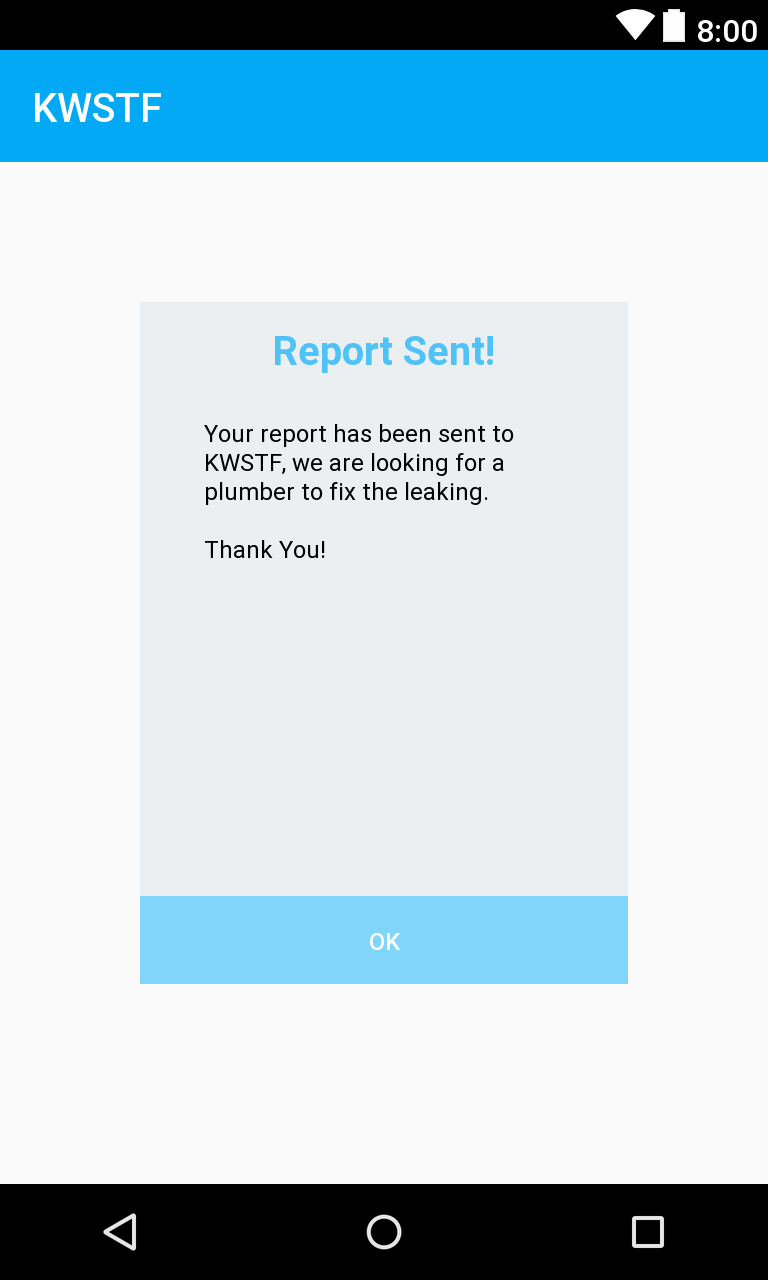
\includegraphics[width=4cm]{files/report_leak/popup.png} }} \\


\subfloat[label 4]{{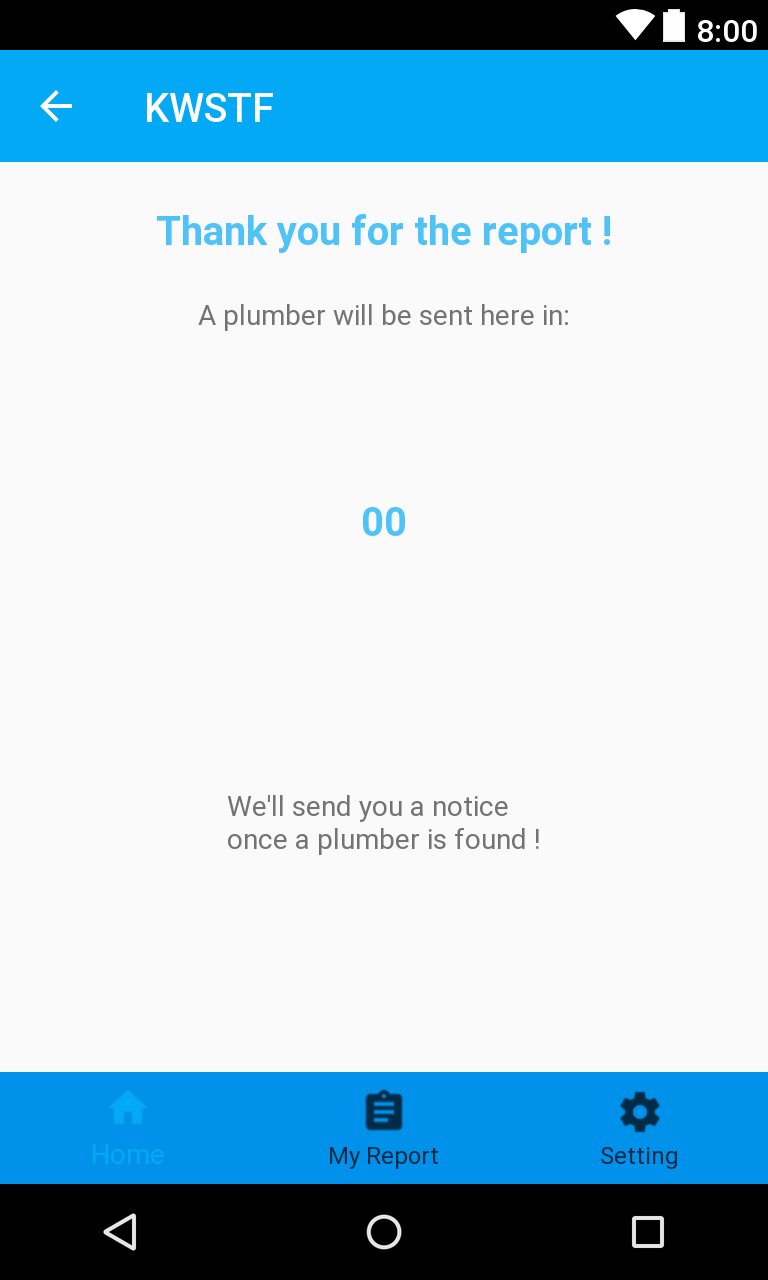
\includegraphics[width=4cm]{files/report_leak/a2.png} }}%
\qquad
    \subfloat[label 5]{{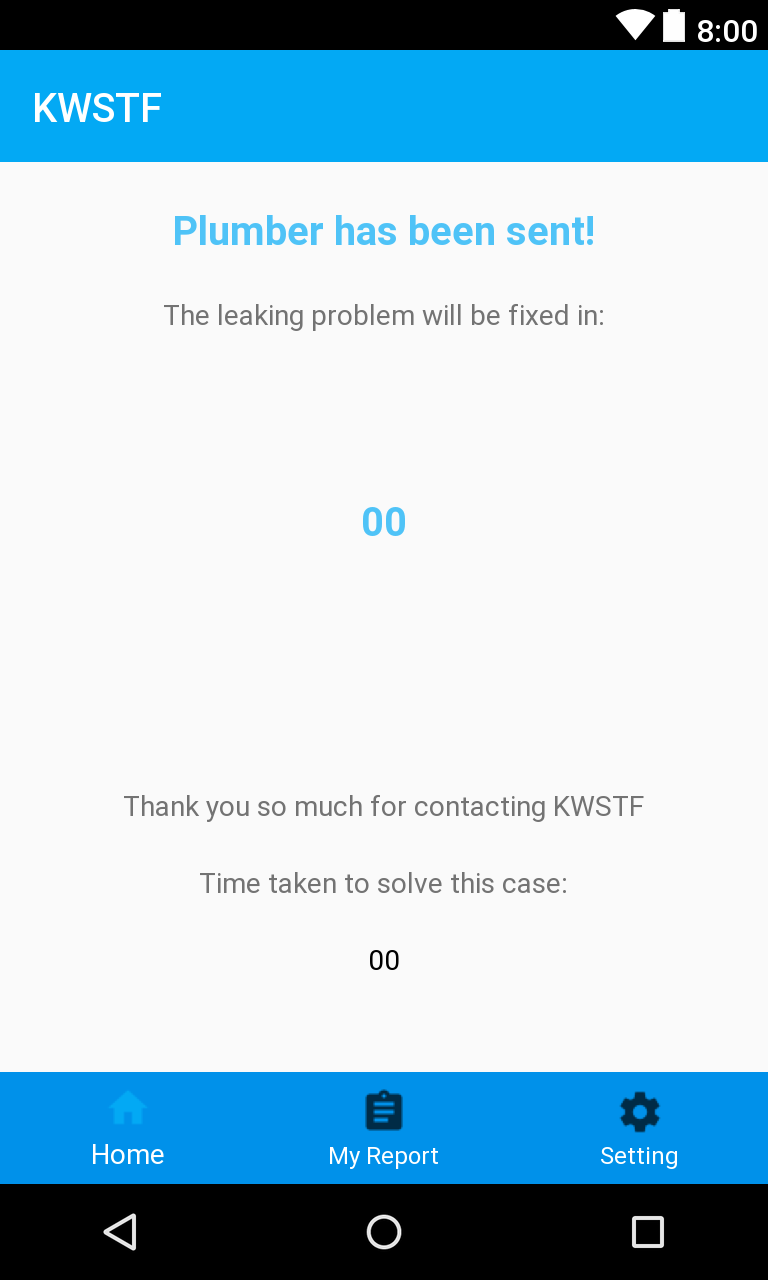
\includegraphics[width=4cm]{files/report_leak/a4.png} }}%
    \caption{Guideline 01: Report Leak}%
\end{figure}

\begin{figure}[H]
  \centering

\subfloat[label 1]{{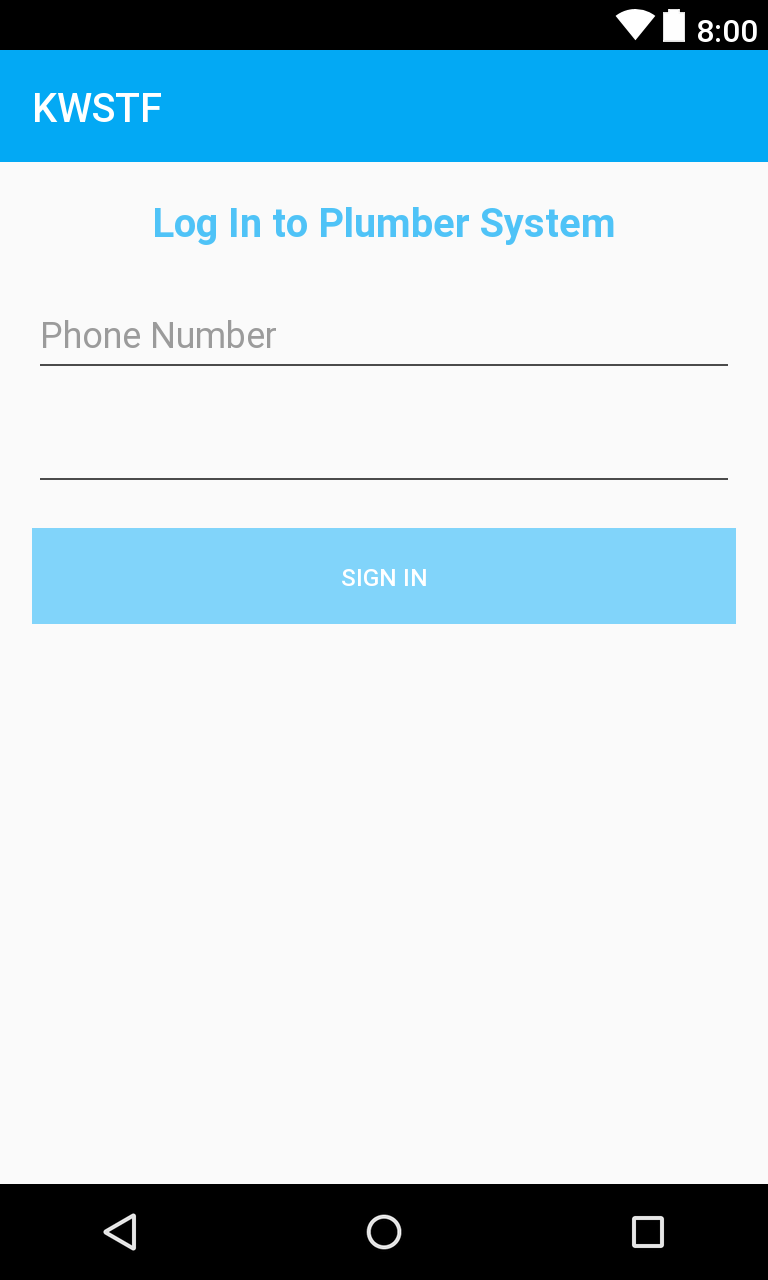
\includegraphics[width=4cm]{files/register/login.png} }}%
\qquad
    \subfloat[label 2]{{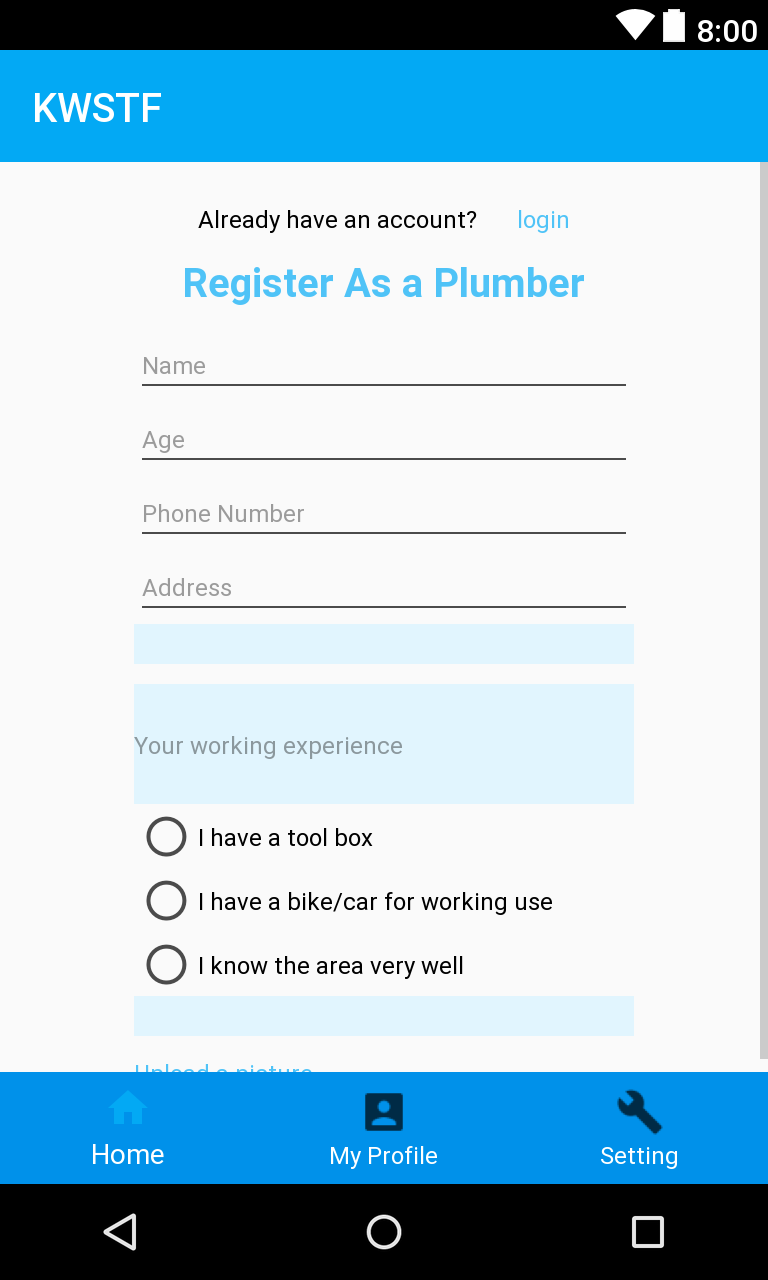
\includegraphics[width=4cm]{files/register/b1.png} }}%
    \qquad
    \subfloat[label 3]{{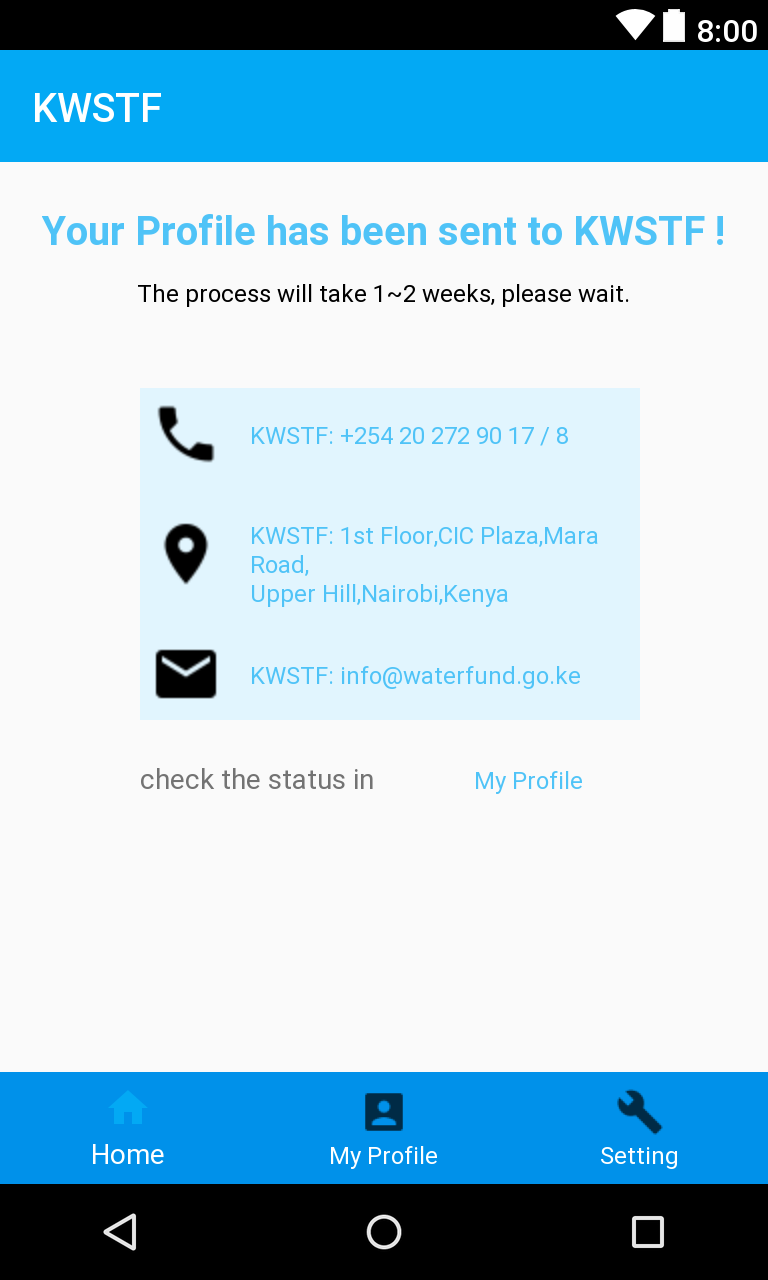
\includegraphics[width=4cm]{files/register/b2.png} }} \\


\subfloat[label 4]{{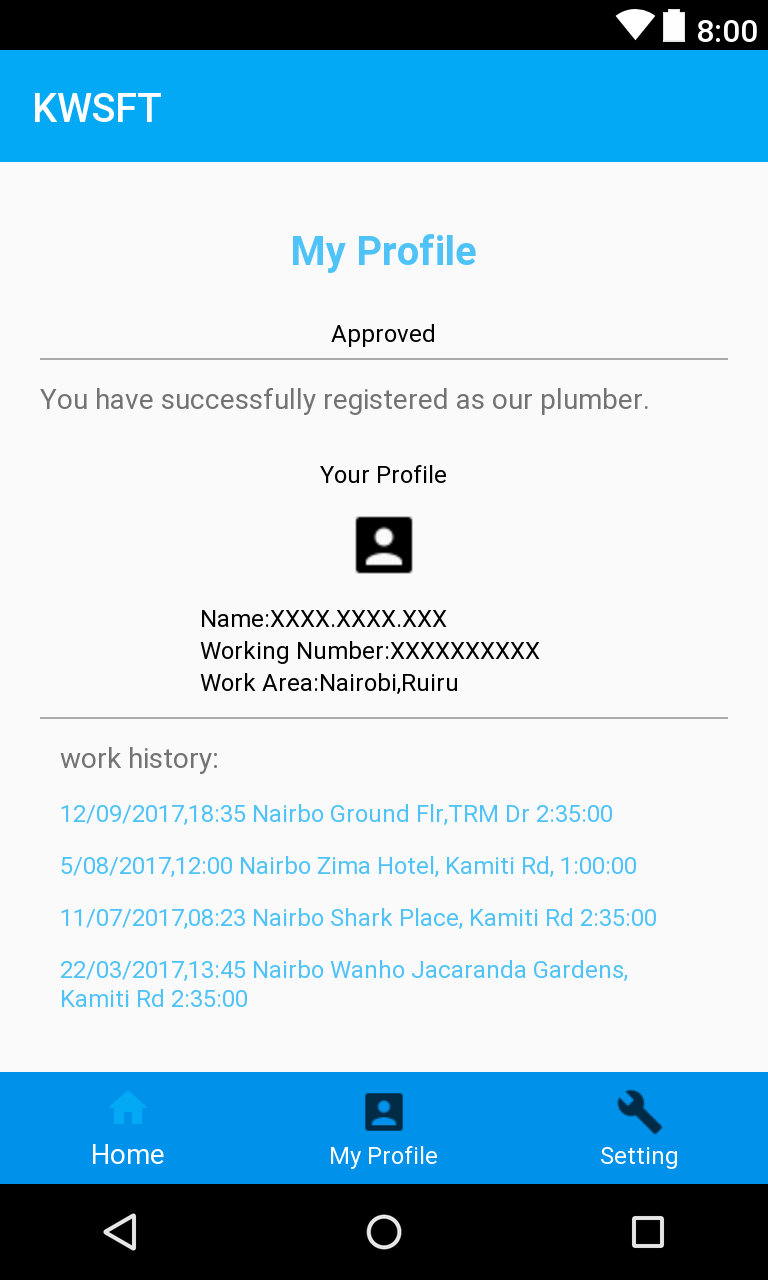
\includegraphics[width=4cm]{files/register/b3.png} }}%
\qquad
    \subfloat[label 5]{{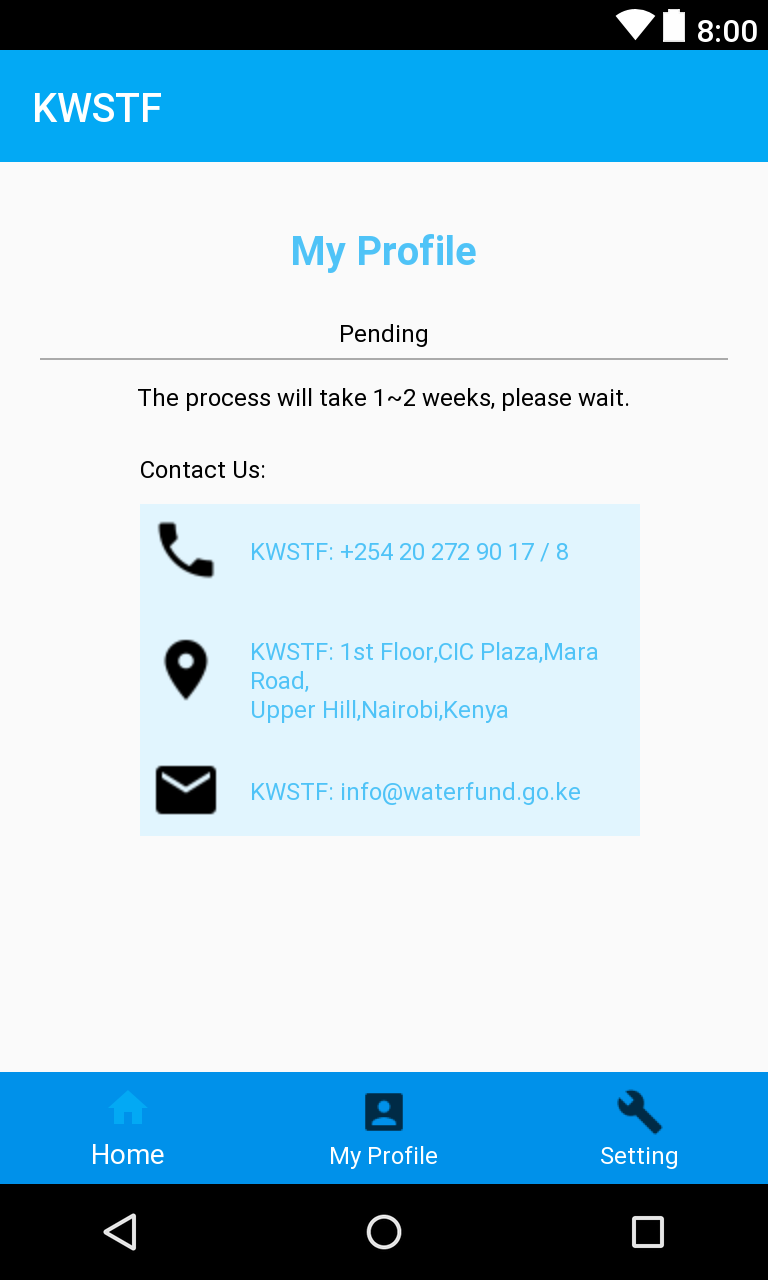
\includegraphics[width=4cm]{files/register/b4.png} }}%
    \qquad
        \subfloat[label 6]{{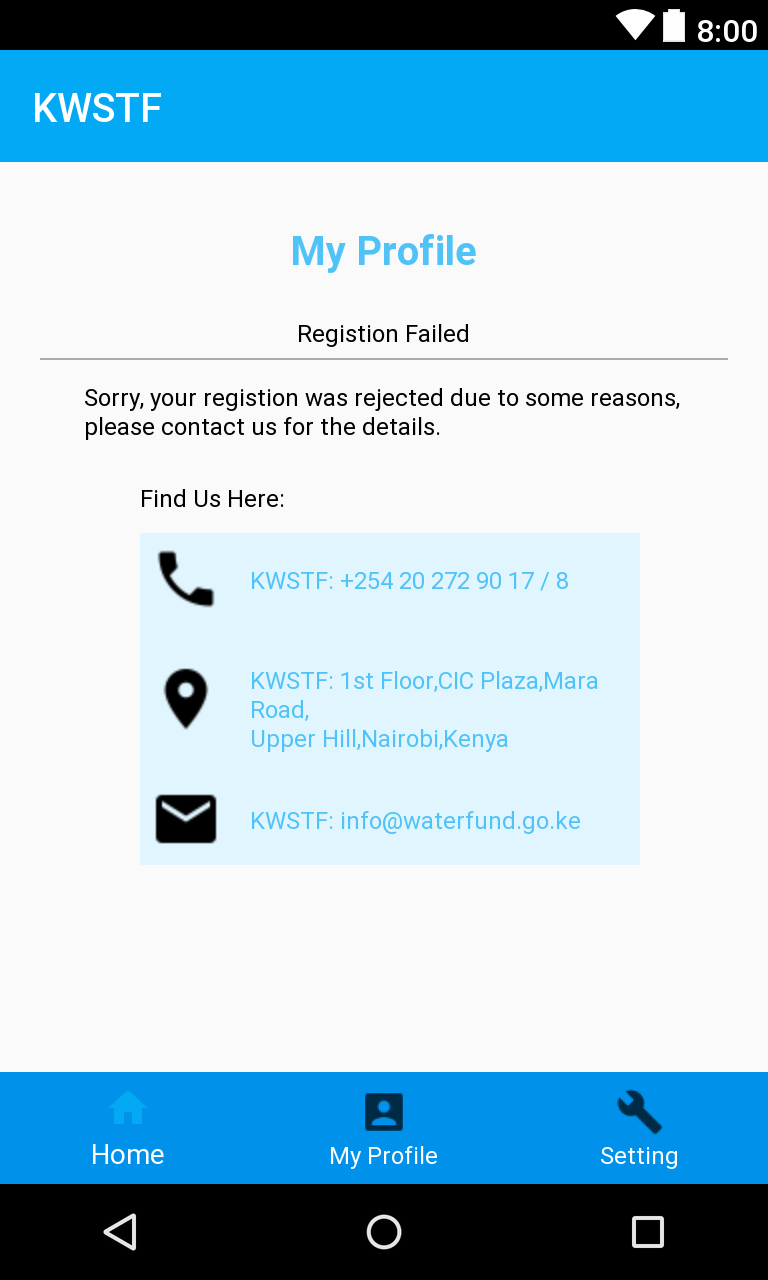
\includegraphics[width=4cm]{files/register/b5.png} }}%
    \caption{Guideline 01: Register as a plumber}%
\end{figure}

\begin{figure}[H]
  \centering

\subfloat[label 1]{{
\includegraphics[width=4cm]{files/menu/about.png} }}%
\qquad
    \subfloat[label 2]{{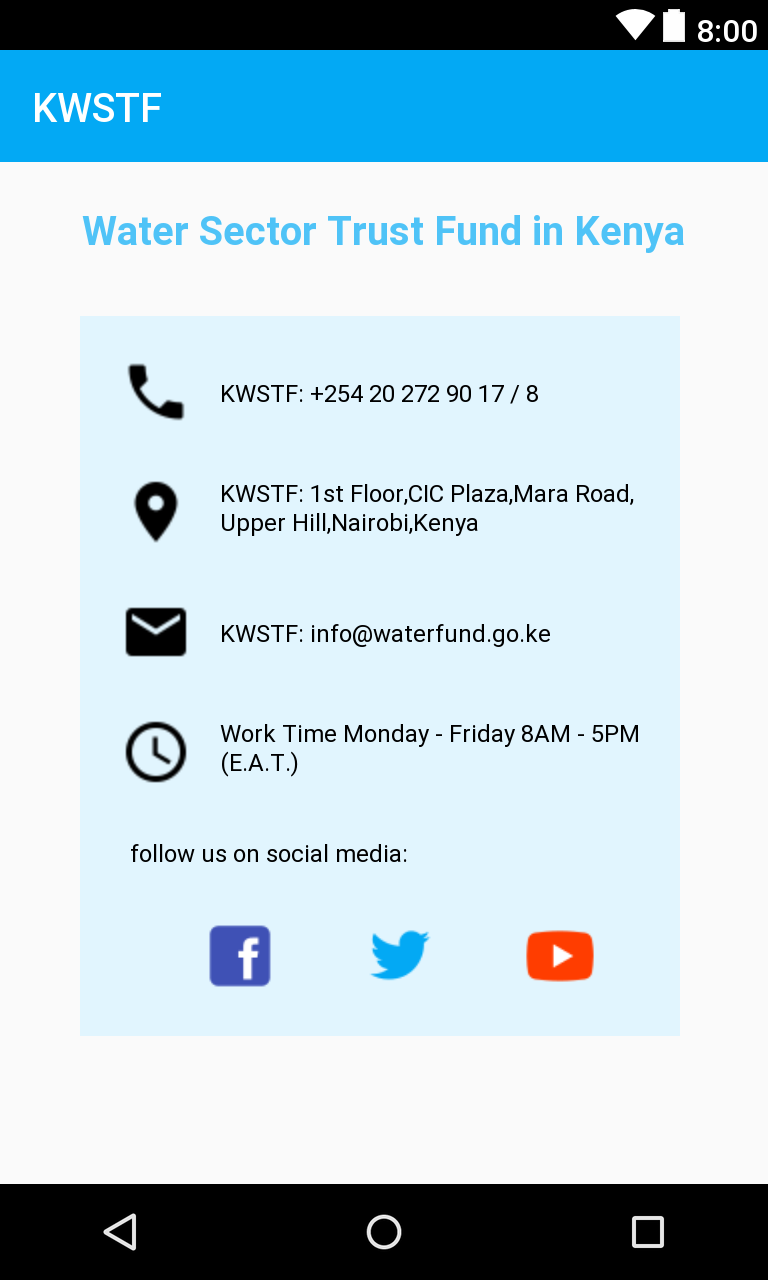
\includegraphics[width=4cm]{files/menu/contact.png} }}%
    \qquad
    \subfloat[label 3]{{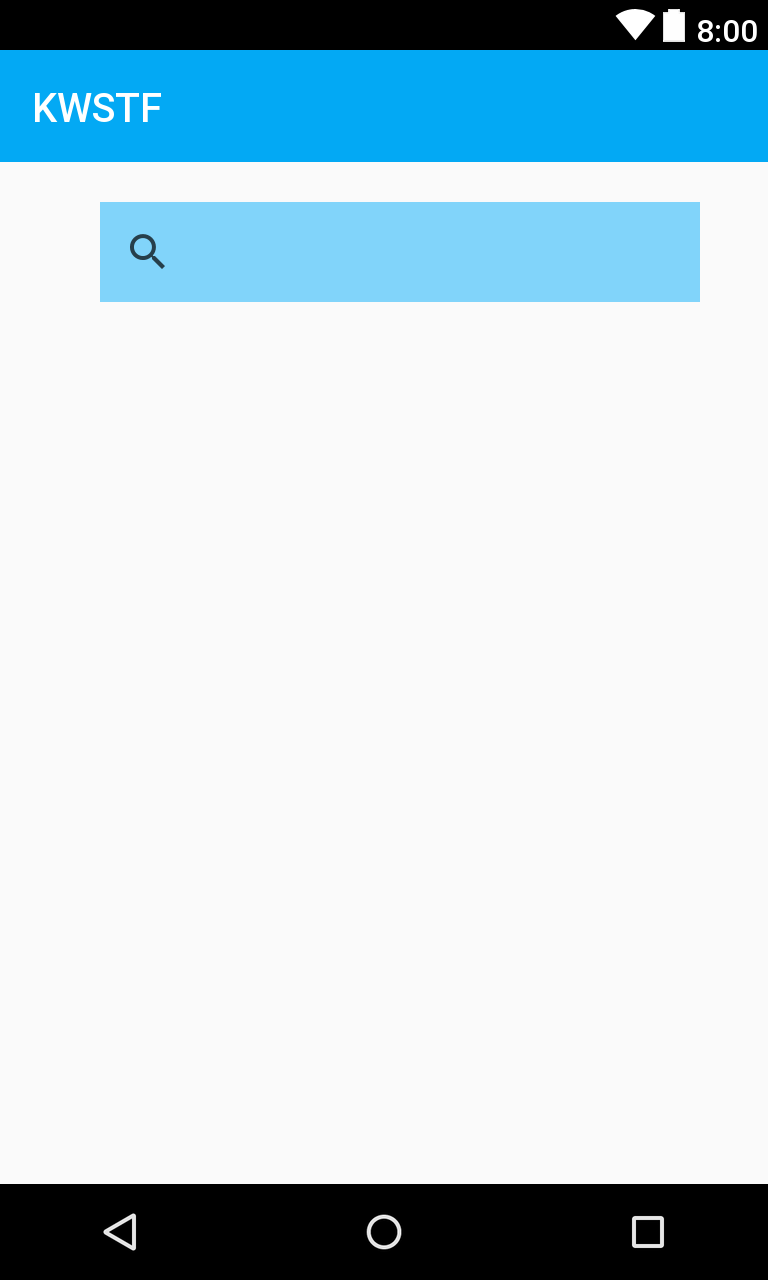
\includegraphics[width=4cm]{files/menu/search.png} }} \\
    \caption{Guideline 01: Menu}%
\end{figure}

\subsection{Guideline 02}
Four Principles of Good Design (Shneiderman 1998):\\
4. User should receive continuous feedback. \\

\noindent
Implementation:
\begin{itemize}
\item Popup-window
\item Time-track and Estimated Time Notice
\end{itemize}
\begin{figure}[H]
\centering
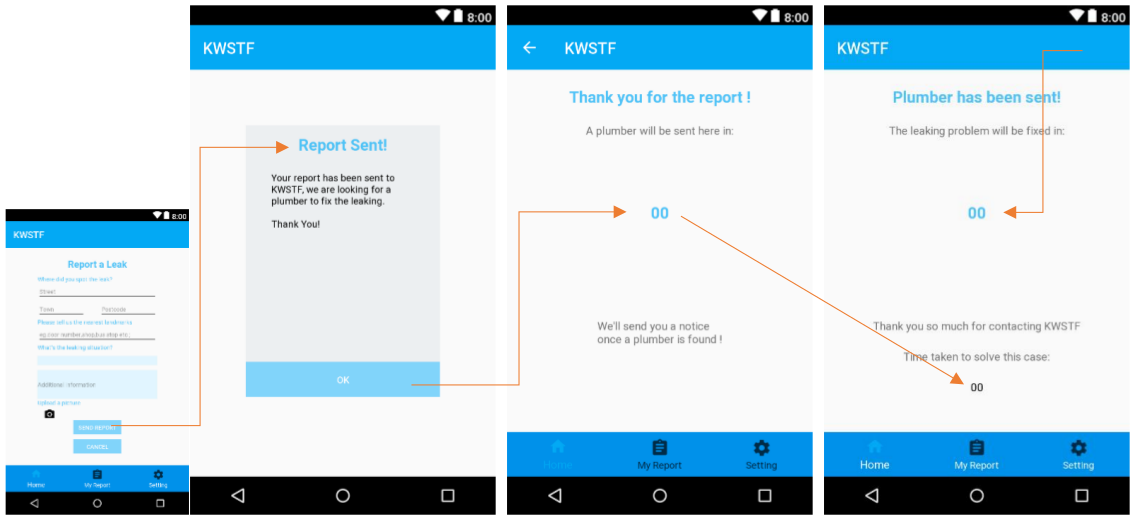
\includegraphics[width=15cm]{files/figures/fig1_guide2.png}
\caption{Guideline 02: When the user want to report a leak and right after the user hit the “Send Report” button, a pop-up window will be
activated and displayed on “My Report” page, give the user positive respond that the report has been sent. At the same
time, the timer was sent to track the time that has passed since the user submitted the case, so the user could have a clear
image that how fast the KWSTF are responding to the report.
After KWSTF has found a plumber, “My Report” will be updated, a “Count-down” timer will be activated according to the
time the plumber estimated to spend on fixing the leak, so the user could be clear that the leak will be fixed in a specific
time. At the same time, the previous timer will stop counting and display the time used to find a plumber.}
\end{figure}



\begin{figure}[H]
\centering
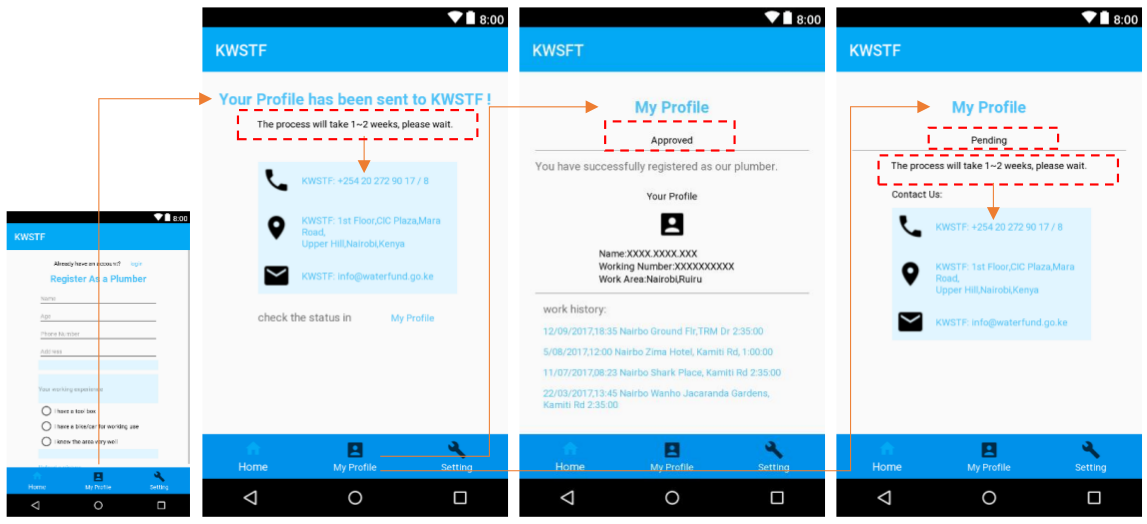
\includegraphics[width=15cm]{files/figures/fig2_guide2.png}
\caption{Guideline 02: After the plumber has submitted the registrations form, the user will be sent to “My Profile”, with a notification on the title saying
the profile has been sent to KWSTF, the estimated time for the process will be displayed under the title, so the user would be clear
when he could get the respond from KWSFT, besides that, the contact information are displayed under, the user could choose to
call or send an email to inquire about his case.
When a decision is made by KWSTF, “My Profile” page will be updated, with “Approved” or “Pending” or “Rejected” status
displayed under, if it’s still in “Pending”, KWSTF contact info are available on the page for user to take the next step.
}
\end{figure}

\subsection{Guideline 03}
Nielsen’s Ten Heuristic Rules (1993):\\
1. Simple and natural dialog 2. Speak the user’s language 3. Minimize user’s memory load 7. Shortcuts

\noindent
Implementation:
\begin{itemize}
\item Bottom Navigation Bar
\item Menu Items
\item Page Update
\end{itemize}

\begin{figure}[H]
\centering
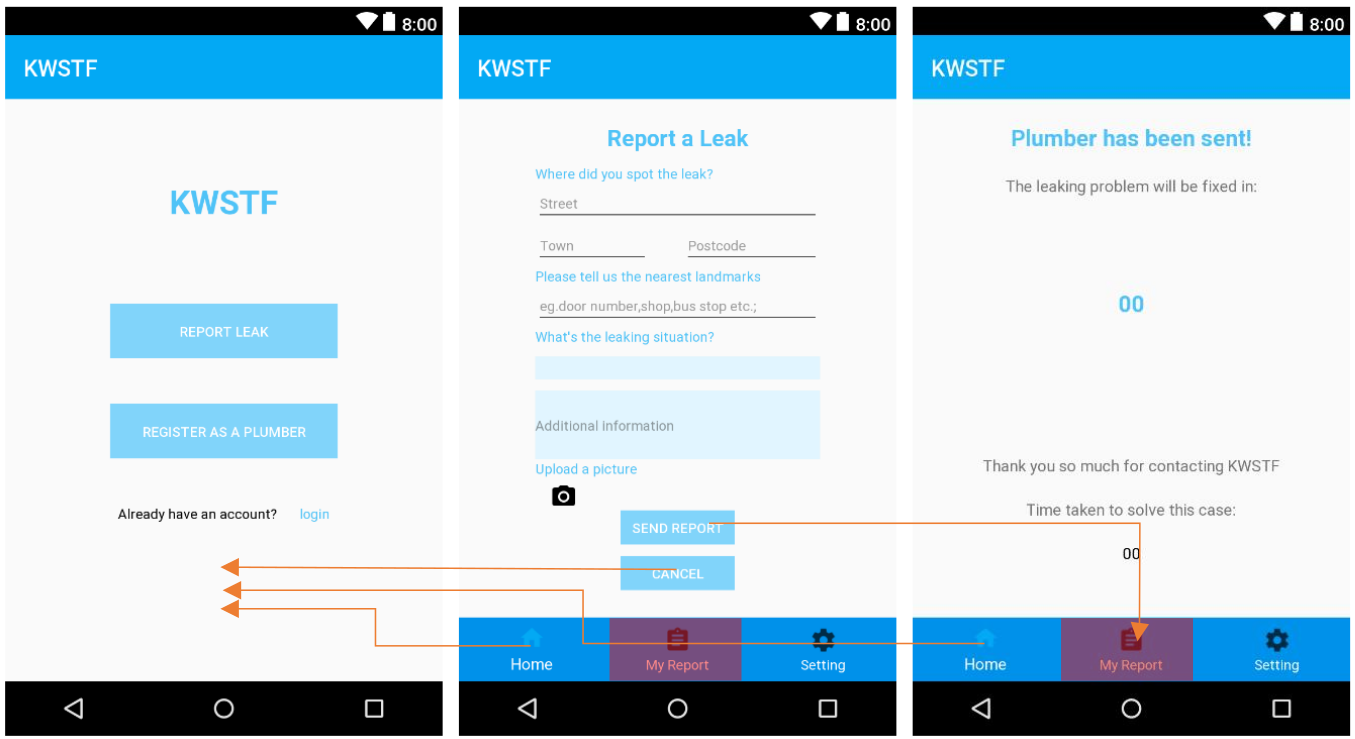
\includegraphics[width=15cm]{files/figures/fig1_guide3.png}
\caption{Guideline 03: The app use user’s language and give users hint with blue text to prevent erros. “Bottom Navigation” bar is the shortcut for the
pages. User can always go back to home page and start over again. After the report was sent, it will be stored in “My Report”,
users could go to the page and check the updates.}
\end{figure}

\begin{figure}[H]
\centering
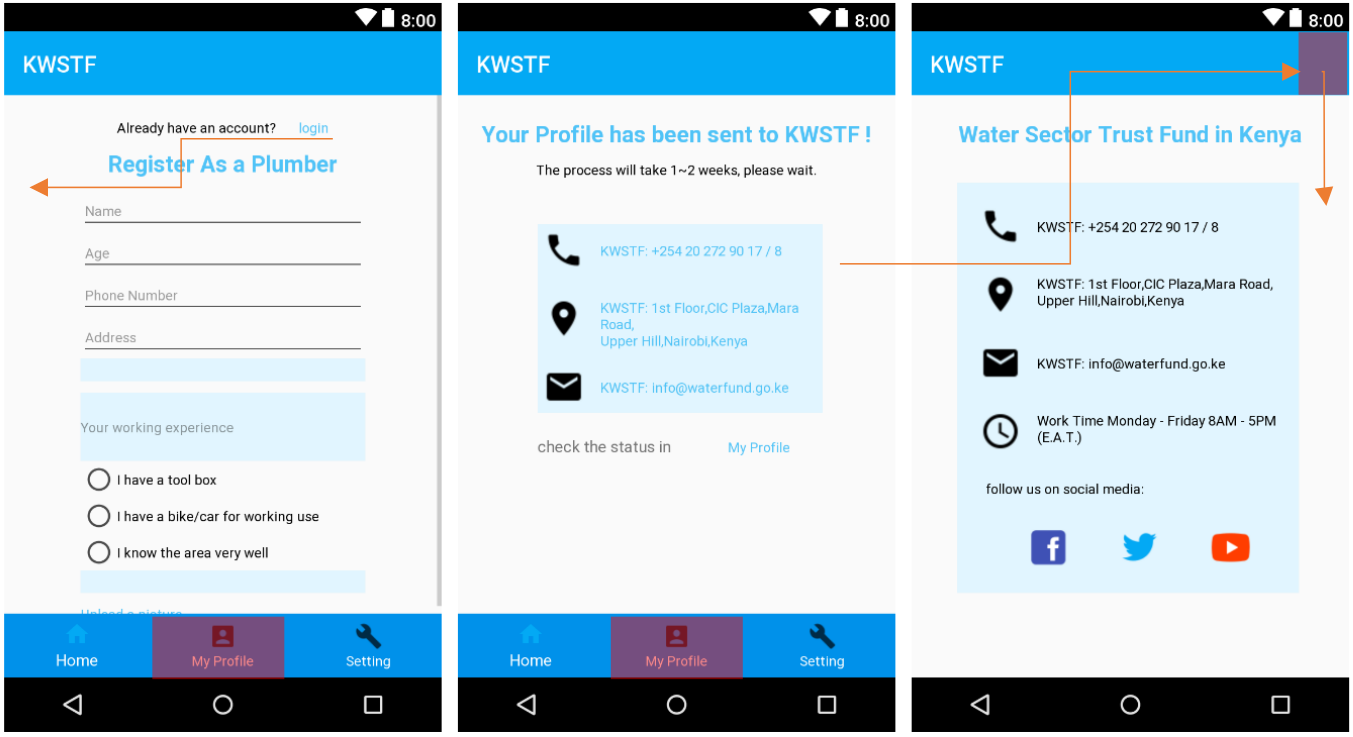
\includegraphics[width=15cm]{files/figures/fig2_guide3.png}
\caption{Guideline 03: “Login” link was listed on top of the page, so if the user already have an account, he can use the shortcut to login. The
KWSTF contact card will be displayed every time there is a need, and the contact info are listed in the menu items, users
can also use “Menu” to quickly locate the contact info.}

\end{figure} 

\subsection{Guideline 04}
Jakob Nielsen’s Ten Usability Heuristics:\\
2. Match between system and the real world (METAPHOR) 6. Recognition rather than recall (MEMORY) 8. Aesthetic and minimalist design (DESIGN)

\noindent
Implementation:
\begin{itemize}
\item Drop-down list
\item Radio Button
\end{itemize}

\begin{figure}[H]
\centering
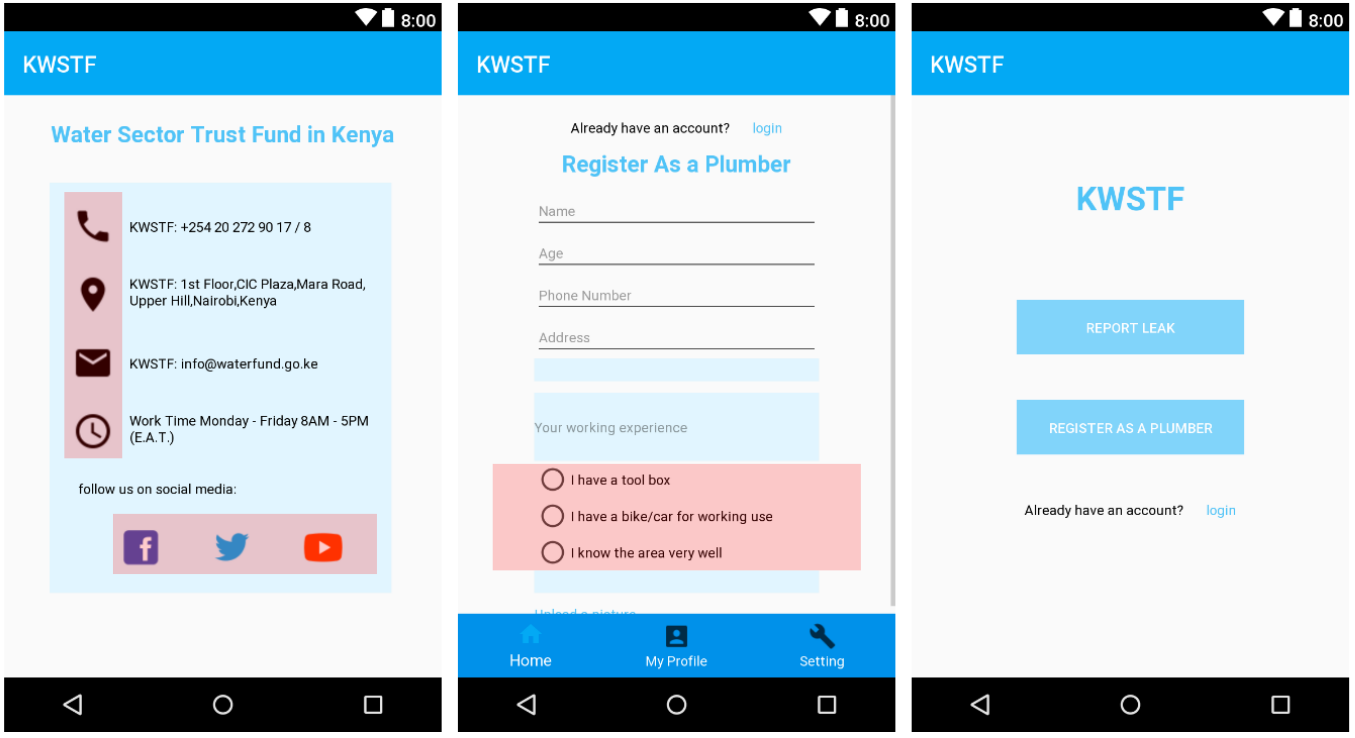
\includegraphics[width=15cm]{files/figures/fig1_guide4.png}
\caption{Guideline 04: A lot of Icons are used to make the app works closely with user’s real life. When we need to have the input from users, we
provide “Dropdown menu” or “Radio Button”, so the users don’t need to recall but only to choose from the current. The
design have only one main theme color: blue, when there is a need to distinguish, different blue tone is used instead of
other colors, which makes the app design is simple and not color-blind users.}\nocite{*}

\end{figure} 



\subsection{Guideline 05}
Smith \& Mosier: Data Display\\
2.0/13 Consistent Wording 2.0/15 Consistent Grammatical Structure
\noindent
Implementation:
\begin{itemize}
\item Grammatical Structure goes like: Report/Register + A leak/ As a plumber
\item Wording goes like: I have/know + tool box/the area
\end{itemize}

\begin{figure}[H]
\centering
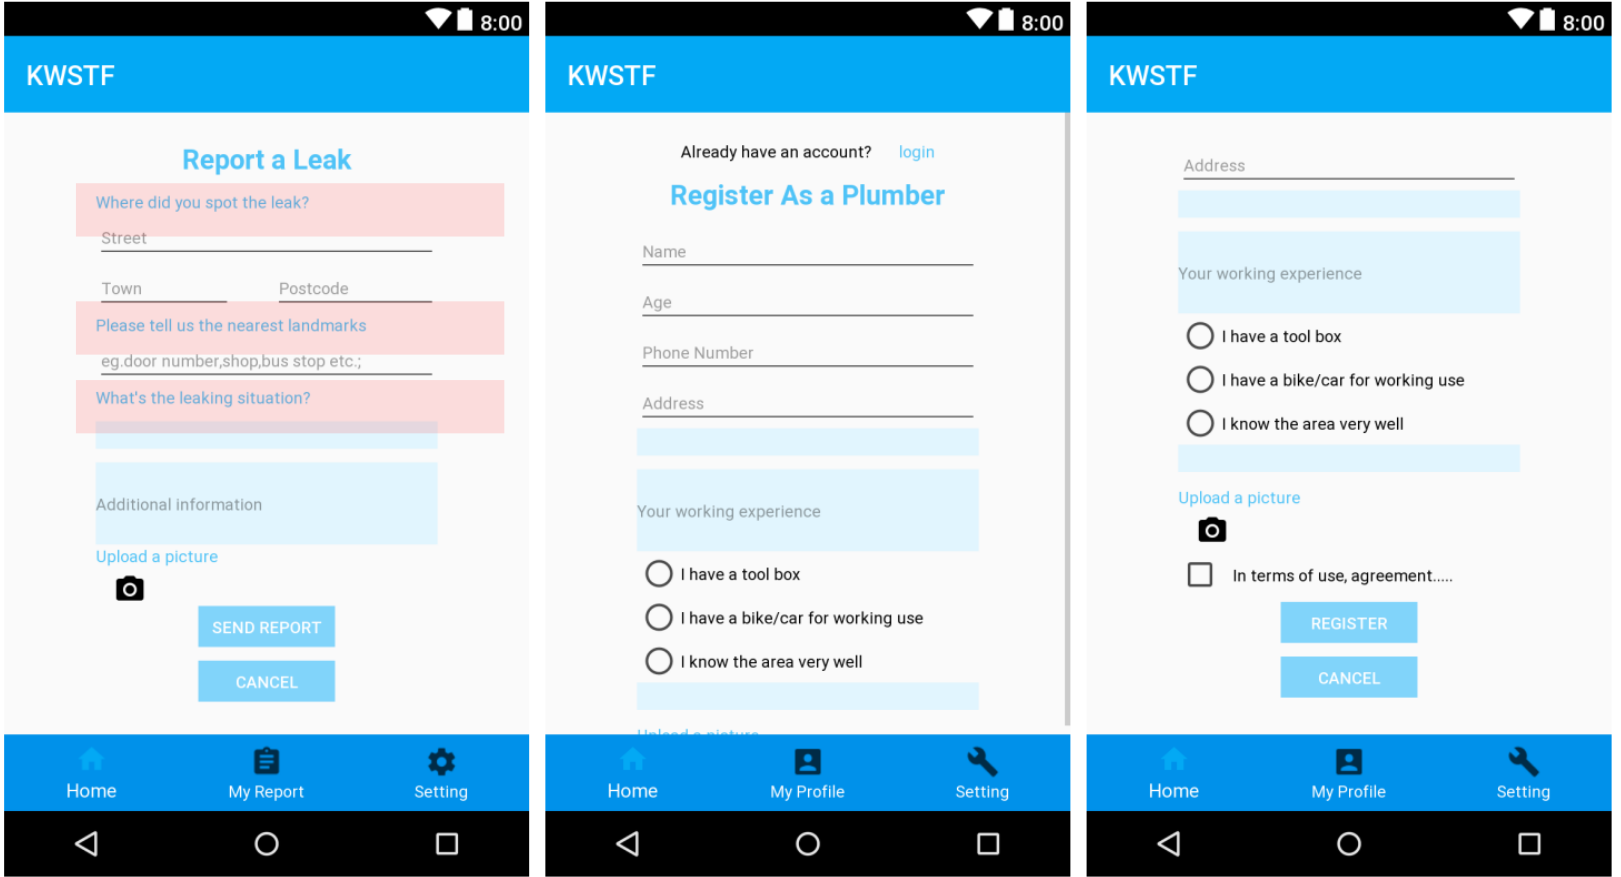
\includegraphics[width=15cm]{files/figures/fig1_guide5.png}
\caption{Guideline 05}

\end{figure} 



\newpage

\bibliographystyle{plain}
\bibliography{ref} 

\end{document}
